% =====================================================================
%  DAT305 - Project 1: Explainable Machine Learning for Gallstone Disease
%  IEEE conference template (IEEEtran).
% =====================================================================
\documentclass[conference]{IEEEtran}
\IEEEoverridecommandlockouts

\usepackage[T1]{fontenc}
\usepackage{cite}
\usepackage{amsmath,amssymb}
\usepackage{graphicx}
\usepackage{booktabs}
\usepackage{xcolor}
\usepackage[hidelinks]{hyperref}

\graphicspath{{figures/}{../figures/}}
\raggedbottom

\begin{document}

\title{Explainable Machine Learning for Gallstone Disease Prediction from Bioimpedance and Laboratory Data}

\author{
\IEEEauthorblockN{Neizan Roggie, Pablo Traverso and Alejandro Mac\'ias}
\IEEEauthorblockA{\textit{DAT305 AI for Engineers -- University of Stavanger}}
}

\maketitle

% ---------------------------------------------------------------------
\begin{abstract}
Gallstone disease is a common condition linked to demographic, metabolic and body-composition factors. Using the UCI Gallstone-1 dataset (319 patients, 38 features), we trained and compared four classifiers (Logistic Regression, Random Forest, SVM and XGBoost) inside a leakage-free scikit-learn pipeline with stratified 5-fold cross-validation. XGBoost obtained the best cross-validated performance (F1 = 0.79, ROC-AUC = 0.85) and reached an accuracy of 0.77 and ROC-AUC of 0.85 on a held-out test set. We explained the model with SHAP and LIME and checked the robustness of the resulting ranking against permutation importance, logistic-regression coefficients and an entropy decision tree. C-reactive protein (CRP) and Vitamin D were the most informative features across SHAP, permutation importance and a decision tree, followed by a group of correlated body-composition variables and liver/lipid markers, in agreement with the reference study.
\end{abstract}

\begin{IEEEkeywords}
gallstone disease, explainable AI, SHAP, LIME, XGBoost, bioimpedance
\end{IEEEkeywords}

% ---------------------------------------------------------------------
\section{Introduction}
Gallstone disease (cholelithiasis) affects a large share of the adult population and is usually diagnosed with abdominal ultrasound. Risk factors include obesity, metabolic syndrome and dyslipidemia, which suggests that routinely collected bioimpedance and laboratory data could help to flag patients at risk. Esen \textit{et al.}~\cite{esen2024} showed that machine-learning models can predict gallstone disease from such data with about 85\% accuracy. However, a high accuracy alone does not explain \emph{why} a model makes a prediction, which limits clinical trust.

The objective of this project is twofold: (i) to build a classifier that distinguishes patients with and without gallstones, and (ii) to identify which clinical characteristics contribute most to its predictions using explainable-AI (XAI) methods.

% ---------------------------------------------------------------------
\section{Methodology}
\subsection{Dataset}
The UCI Gallstone-1 dataset~\cite{uci} contains 319 outpatients from Ankara VM Medical Park (2022--2023), 161 with gallstones and 158 without, with no missing values. Its 38 features cover demographics (age, sex, height, weight, BMI), comorbidities, bioimpedance (body water, muscle and fat mass, protein, visceral fat, hepatic fat) and laboratory tests (glucose, lipids, AST/ALT/ALP, creatinine, GFR, CRP, hemoglobin, Vitamin D). Following the UCI documentation, the target was recoded so that $1=$ gallstones (disease) and $0=$ healthy.

\subsection{Preprocessing and models}
The data were split into a stratified training set (80\%, 255 patients) and test set (20\%, 64 patients). The 33 continuous features were standardized with \texttt{StandardScaler} inside a \texttt{ColumnTransformer}, while the 5 binary features were passed through unchanged. Scaler and classifier were wrapped in a single \texttt{Pipeline} so that the scaler is fitted only on training folds, avoiding data leakage. Four classifiers with default hyperparameters were compared with stratified 5-fold cross-validation: Logistic Regression (LR), Random Forest (RF), Support Vector Machine (SVM) and XGBoost. The model with the best mean cross-validated F1-score was selected; all four models were then refitted on the whole training set and evaluated on the held-out test set.

\subsection{Explainability}
We used \texttt{shap.TreeExplainer}~\cite{lundberg2017,lundberg2020}, which computes exact SHAP values for tree ensembles, to obtain global (beeswarm and mean $|$SHAP$|$) and local (waterfall) explanations on the 64 test patients. LIME~\cite{ribeiro2016} was applied to the same three representative patients (a true positive, a false negative and a false positive) to compare both local explanations. Finally, the robustness of the global ranking was assessed against permutation importance (ROC-AUC drop, 30 repeats), the absolute LR coefficients and a depth-4 decision tree trained with the entropy criterion.

% ---------------------------------------------------------------------
\section{Results and Explainability}
\subsection{Classification performance}
Table~\ref{tab:results} summarizes the results. XGBoost obtained the best cross-validated F1-score and ROC-AUC and was selected. On the test set it reached an accuracy of 0.77, recall (sensitivity) of 0.78, specificity of 0.75 and ROC-AUC of 0.85 (TP\,=\,25, TN\,=\,24, FP\,=\,8, FN\,=\,7). Logistic Regression scored slightly higher on the 64-patient test set (F1\,=\,0.81), but the difference lies within the cross-validation standard deviation ($\approx$0.05), so the model selection was kept as decided a priori.

\begin{table}[t]
\caption{Classifier performance: 5-fold CV on the training set (mean $\pm$ std) and held-out test set.}
\label{tab:results}
\centering
\setlength{\tabcolsep}{3.5pt}
\begin{tabular}{@{}lcccc@{}}
\toprule
 & \multicolumn{2}{c}{\textbf{5-fold CV}} & \multicolumn{2}{c}{\textbf{Test set}}\\
\cmidrule(lr){2-3}\cmidrule(lr){4-5}
\textbf{Model} & F1 & ROC-AUC & F1 & ROC-AUC\\
\midrule
\textbf{XGBoost} & $\mathbf{0.79\pm0.05}$ & $\mathbf{0.85\pm0.04}$ & 0.77 & 0.85\\
Logistic Reg. & $0.77\pm0.04$ & $0.83\pm0.04$ & \textbf{0.81} & \textbf{0.88}\\
Random Forest & $0.76\pm0.10$ & $0.83\pm0.05$ & 0.72 & 0.84\\
SVM & $0.69\pm0.08$ & $0.79\pm0.08$ & 0.72 & 0.81\\
\bottomrule
\end{tabular}
\end{table}

\subsection{Global explanations}
Fig.~\ref{fig:beeswarm} shows the SHAP summary plot. CRP is by far the most important feature (mean $|$SHAP$|=1.90$), followed by Vitamin D (0.81), body protein content (0.59), AST (0.54) and LDL (0.46); ALP, visceral fat rating, obesity (\%), GFR and visceral fat area complete the top 10. SHAP values reconstruct the model output exactly (maximum error $1.2\times10^{-7}$).

CRP is ranked first by SHAP, permutation importance and the decision tree, which also ranks Vitamin D second; CRP and AST are the only features in the top 10 of SHAP, permutation importance and LR simultaneously. Beyond the top two, the rankings agree only moderately (Spearman $\rho=0.30$ between SHAP and permutation importance, $\approx0$ with LR). This is explained by strong collinearity among the body-composition features (12 of 78 pairs with $|r|>0.8$), whose importance is shared differently by tree and linear models.

\begin{figure}[t]
\centering
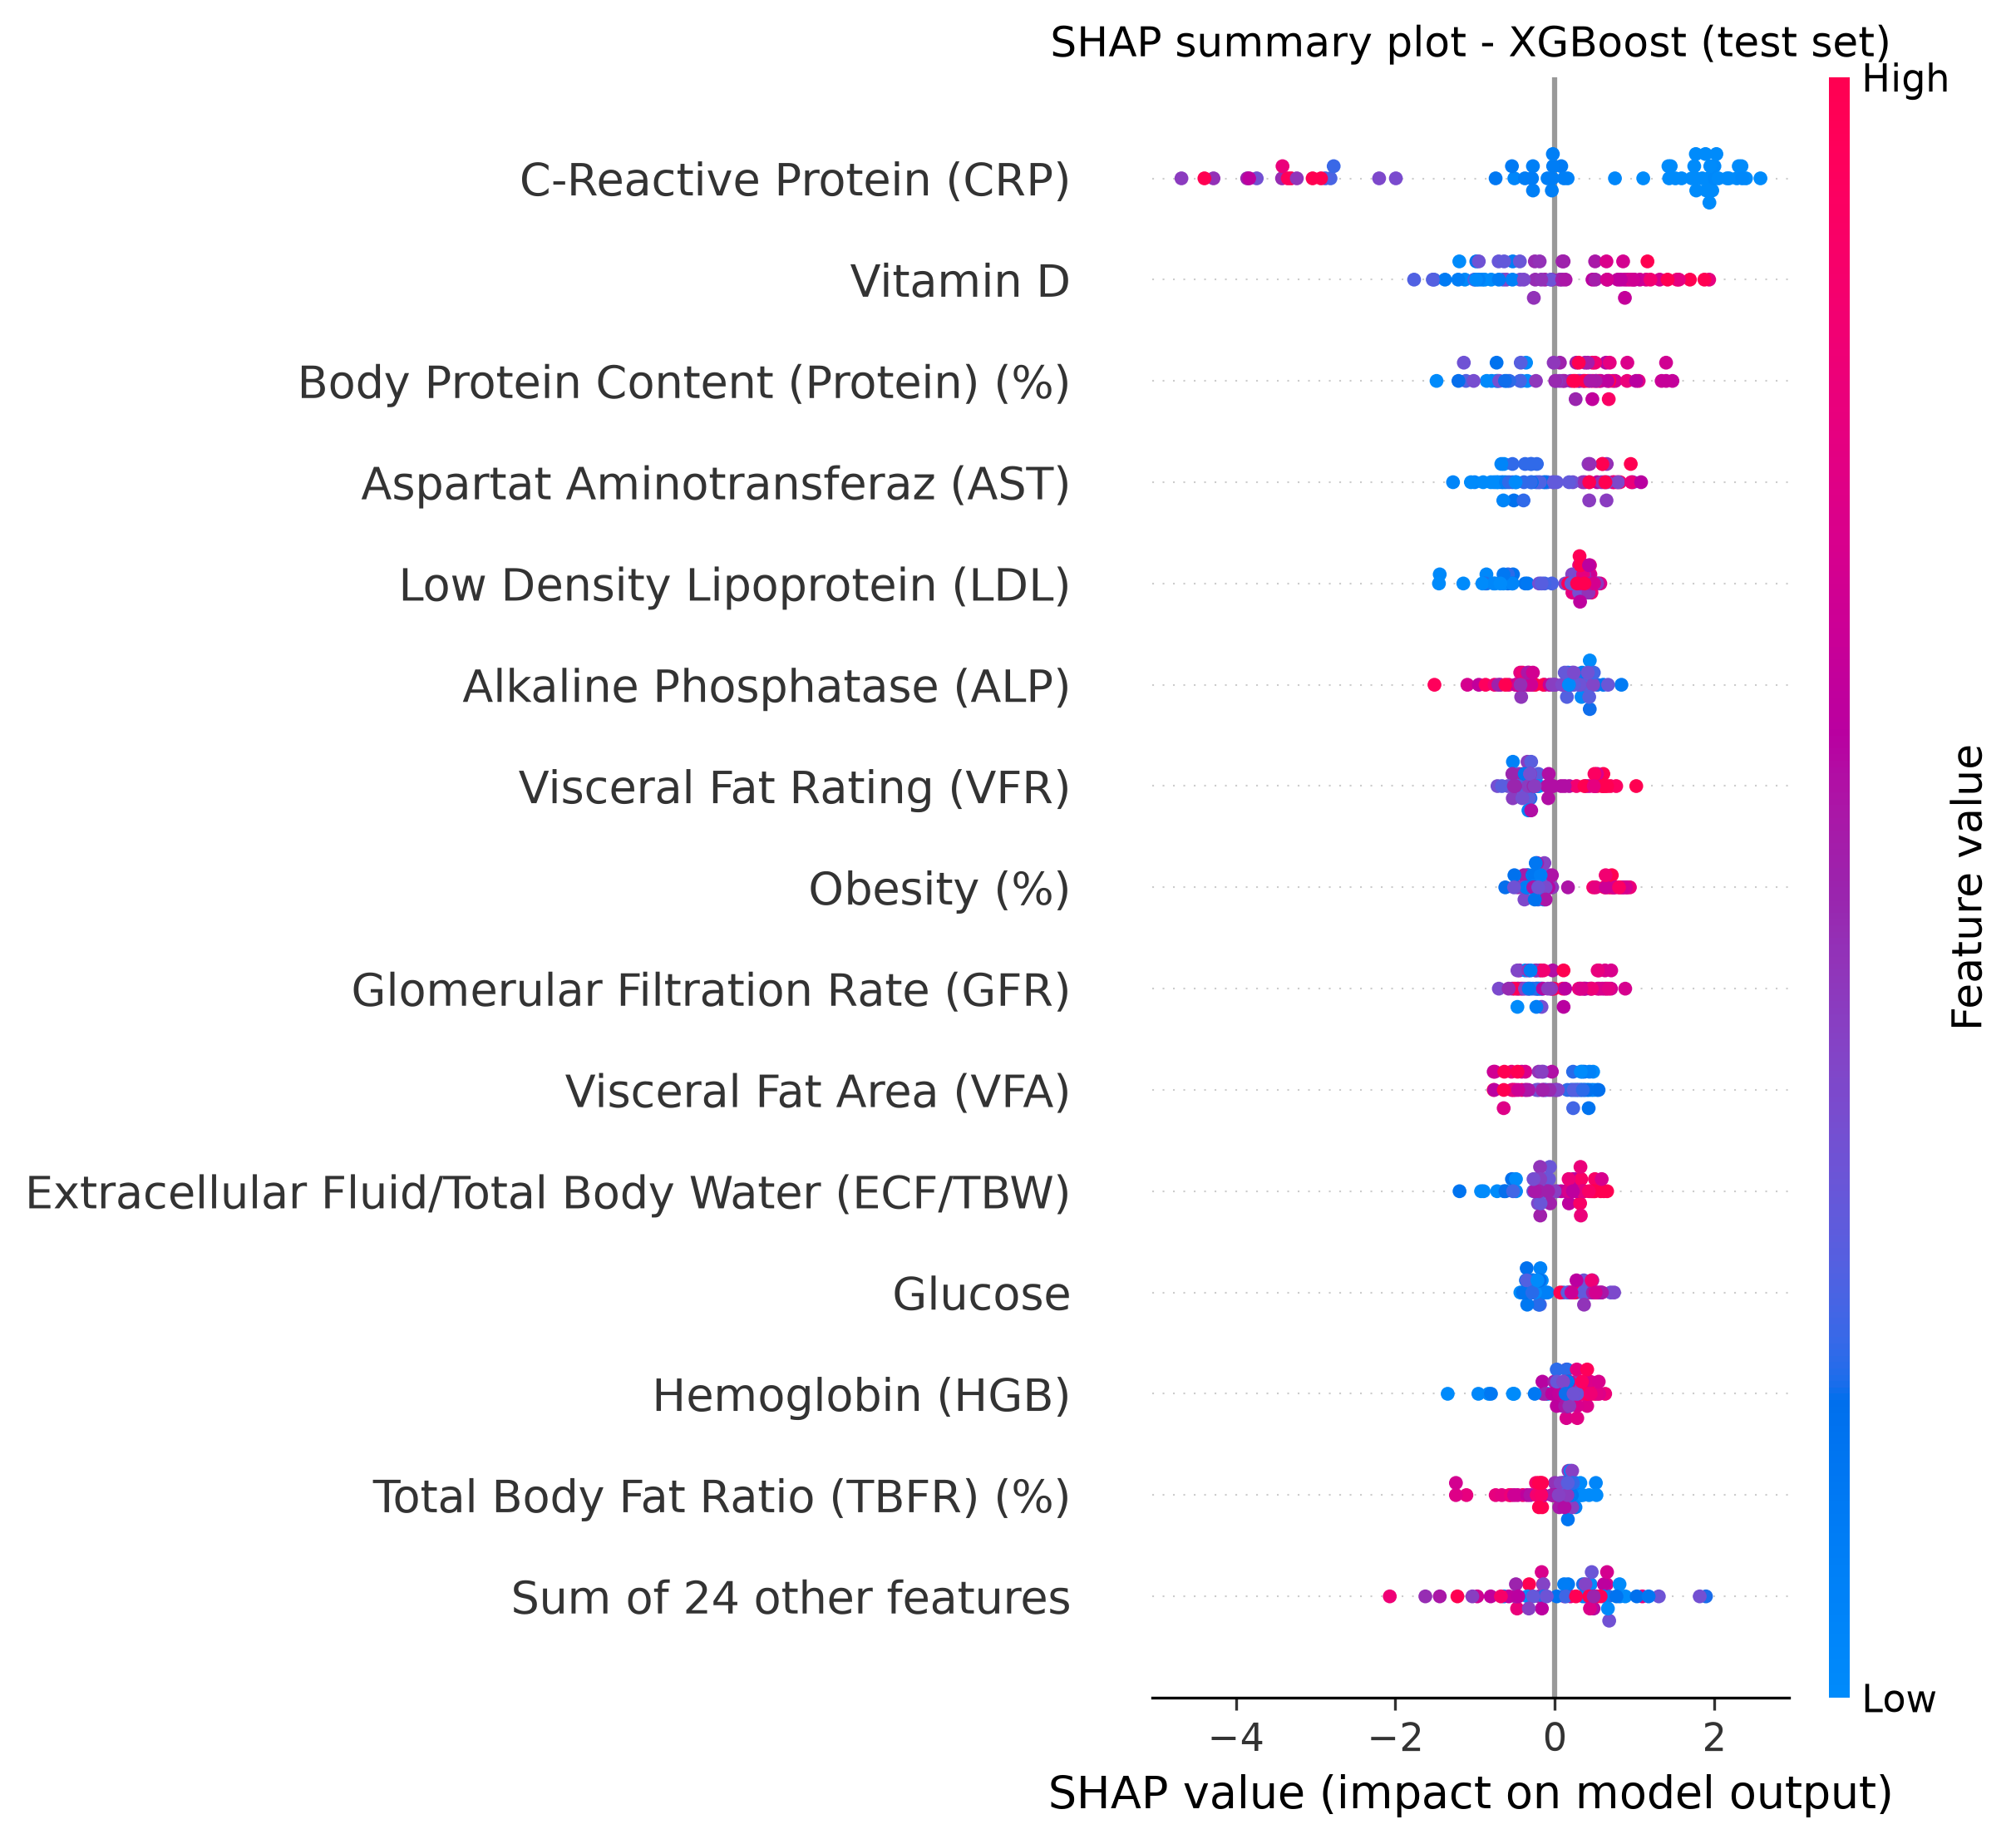
\includegraphics[width=0.92\columnwidth]{shap_beeswarm.png}
\caption{SHAP summary plot of XGBoost on the test set. Each dot is a patient; positive SHAP values push the prediction towards gallstone disease. Colour encodes the feature value.}
\label{fig:beeswarm}
\end{figure}

\subsection{Local explanations}
For the three selected patients, SHAP and LIME share 3--4 of their top-5 features. The most confident false negative (P(disease)\,=\,0.02) is driven towards ``healthy'' by low AST, a high body-fat ratio, low Vitamin D and low LDL, i.e.\ a gallstone patient whose laboratory profile resembles the control group. LIME's local linear fits are weak ($R^2=0.15$--$0.36$), so its explanations should be read as approximate.

% ---------------------------------------------------------------------
\section{Discussion and Contributions}
\subsection{Discussion}
Our two most important features, CRP and Vitamin D, coincide with those highlighted by Esen \textit{et al.}~\cite{esen2024} and by other studies on the same dataset~\cite{bart2025}. Our untuned XGBoost reaches the same AUC (0.85) as their best model, with lower accuracy (0.77 vs.\ 0.85). The direction of the effects, however, needs caution: under the UCI encoding, higher CRP is associated with the \emph{healthy} group (mean 3.27 vs.\ 0.46\,mg/L) and higher Vitamin D with gallstones, contrary to clinical expectation. The control group consists of outpatients of the same internal-medicine clinic, not healthy volunteers, which may explain this pattern; moreover, the reference paper uses the opposite label encoding. We therefore report CRP and Vitamin D as the most \emph{informative} features without claiming a causal direction.

The main limitations are the small single-centre sample (64 test patients, no external validation), the absence of hyperparameter tuning, correlated body-composition features that make individual ranks unstable, and the fact that SHAP explains the model, not the disease. The model is a research exercise, not a validated clinical tool. Future work includes hyperparameter optimization, repeated or nested cross-validation and grouping of correlated features before explanation.

\subsection{Individual contributions}
\textbf{Neizan Roggie:} data loading, EDA, preprocessing pipeline, stratified cross-validation, training and evaluation of the four classifiers and export of the selected model.

\textbf{Pablo Traverso:} SHAP and LIME explanations, dependence plots, robustness analysis of the feature ranking, clinical interpretation and contrast with the literature.

\textbf{Alejandro Mac\'ias:} writing of this IEEE report, design of the presentation slides and video, and coordination of the final submission package.

The code is available at \url{https://github.com/taro-py/gallstone-ml-xai}.

% ---------------------------------------------------------------------
\begin{thebibliography}{00}
\bibitem{esen2024} I. Esen, H. Arslan, S. A. Esen, M. G\"ul\c{s}en, N. K\"ultekin, and O. \"Ozdemir, ``Early prediction of gallstone disease with a machine learning-based method from bioimpedance and laboratory data,'' \textit{Medicine}, vol.~103, no.~8, e37258, 2024, doi:10.1097/MD.0000000000037258.
\bibitem{uci} ``Gallstone,'' UCI Machine Learning Repository, 2024. [Online]. Available: https://archive.ics.uci.edu/dataset/1150/gallstone-1
\bibitem{lundberg2017} S. M. Lundberg and S.-I. Lee, ``A unified approach to interpreting model predictions,'' in \textit{Proc. NeurIPS}, 2017, pp.~4765--4774.
\bibitem{lundberg2020} S. M. Lundberg \textit{et al.}, ``From local explanations to global understanding with explainable AI for trees,'' \textit{Nat. Mach. Intell.}, vol.~2, pp.~56--67, 2020.
\bibitem{ribeiro2016} M. T. Ribeiro, S. Singh, and C. Guestrin, ```Why should I trust you?': Explaining the predictions of any classifier,'' in \textit{Proc. 22nd ACM SIGKDD}, 2016, pp.~1135--1144.
\bibitem{bart2025} C. Chakraborty and N. Mukherjee, ``Bayesian hybrid machine learning of gallstone risk,'' arXiv:2506.14561, 2025.
\end{thebibliography}

\end{document}
